\documentclass[twocolumn,times]{aastex631}
\usepackage{acronym}
\usepackage{amsmath}
\usepackage{mathtools}

% \received{March 1, 2021}
% \revised{April 1, 2021}
% \accepted{\today}
% \submitjournal{AJ}
\shorttitle{M$^4$OPT}
\shortauthors{Singer et al.}

% Some of these acronym definitions contain the definite article ("the") and some do not.
% If an acronym's part of speech is a proper noun, then it has a definite article when it
% appears in expanded form. For example, we write "The UltraViolet Explorer is a space telescope,"
% and "UVEX is a space telescope," but we don't write "The luminosity function of the kilonovae is given in Eq. (3)."
\acrodef{ACCESS}[ACCESS]{Advanced Cyberinfrastructure Coordination Ecosystem: Services \& Support}
\acrodef{CDF}[CDF]{cumulative distribution function}
\acrodef{CSR}[CSR]{concept study report}
\acrodef{ETC}[ETC]{exposure time calculator}
\acrodef{FoR}[FoR]{field of regard}
\acrodefplural{FoR}[FoRs]{fields of regard}
\acrodef{FOV}[FOV]{field of view}
\acrodefplural{FOV}[FOVs]{fields of view}
\acrodef{GSFC}[GSFC]{Goddard Space Flight Center}
\acrodef{GRB}[GRB]{gamma-ray burst}
\acrodef{GW}[GW]{gravitational wave}
\acrodef{KN}[KN]{kilonova}
\acrodefplural{KN}[KNe]{kilonovae}
\acrodef{LIGO}[LIGO]{the Laser Interferometer Gravitational-Wave Observatory}
\acrodef{LP}[LP]{linear programming}
\acrodef{MWC}[MWC]{maximum weighted coverage problem}
\acrodef{MIDEX}[MIDEX]{Medium-Class Explorer}
\acrodef{MILP}[MILP]{mixed integer linear programming}
\acrodef{MoO}[MoO]{Mission of Opportunity}
\acrodef{M4OPT}[M$^4$OPT]{the Multi-Mission Multi-Messenger Observation Planning Toolkit}
\acrodef{NOSA}[NOSA]{NASA Open Source Agreement}
\acrodef{NS}[NS]{neutron star}
\acrodef{NSF}[NSF]{the U.S. National Science Foundation}
\acrodef{NUV}[NUV]{near ultraviolet}
\acrodef{FUV}[FUV]{far ultraviolet}
\acrodef{PSF}[PSF]{point spread function}
\acrodef{ROI}[ROI]{region of interest}
\acrodef{SADA}[SADA]{solar array drive assembly}
\acrodef{SN}[SN]{supernova}
\acrodefplural{SN}[SNe]{supernovae}
\acrodef{S/N}[S/N]{signal to noise ratio}
\acrodef{SDSC}[SDSC]{the San Diego Supercomputing Center}
\acrodef{ToO}[ToO]{target of opportunity}
\acrodefplural{ToO}[ToOs]{targets of opportunity}
\acrodef{UV}[UV]{ultraviolet}
\acrodef{UVEX}[UVEX]{the UltraViolet EXplorer}

\begin{document}

\title{Mixed Integer Linear Programming for Time-Domain and Multimessenger Observation Scheduling}

\author[0000-0001-9898-5597]{Leo P. Singer}
\affiliation{Astroparticle Physics Laboratory, NASA Goddard Space Flight Center}
\email{leo.p.singer@nasa.gov}

\author{Friends}
\noaffiliation

\begin{abstract}
\Ac{UVEX} is a wide-field, all-sky, time-domain, ultraviolet survey space telescope selected as a NASA \ac{MIDEX} mission for launch in 2030. \ac{UVEX} will conduct an unprecedented all-sky time-domain survey in two \ac{UV} filters. \ac{UVEX} will follow up \ac{GW} binary neutron star mergers as \acp{ToO}, rapidly scanning across their localization regions to search for their \ac{KN} counterparts. Early-time multiband ultraviolet light curves of \acp{KN} are key to explaining the interplay between jet and ejecta in binary neutron star mergers. Owing to high Galactic extinction in the ultraviolet and \ac{UVEX}'s large \ac{FOV}, variation in sensitivity across the \ac{GW} \ac{ROI} is an important consideration for observation planning. We present an adaptive strategy for \ac{GW} follow-up with \ac{UVEX} in which exposure time is adjusted dynamically for each field individual to maximize the overall probability of detection. We have implemented this strategy in an open source astronomical scheduling toolkit called \ac{M4OPT}, on GitHub at \url{https://github.com/m4opt/m4opt}.
\end{abstract}

\keywords{Computational methods~(1965) --- Gravitational wave astronomy~(675) --- Open source software~(1866) --- Ultraviolet observatories~(1739) --- Ultraviolet transient sources~(1854) --- Wide-field telescopes~(1800)}

\acresetall

\section{Introduction} \label{sec:intro}

In 2017, \ac{LIGO} and Virgo \citep{2017PhRvL.119p1101A} detected a long-duration \ac{GW} inspiral signal, GW170817, at the same time that Fermi \citep{2017ApJ...848L..14G} and INTEGRAL \citep{2017ApJ...848L..15S} recorded a short \ac{GRB}, GRB170817a. The alert sprang traps that had been set by hundreds of telescopes worldwide \citep{2014ApJS..211....7A,2016ApJ...826L..13A} which quickly found the optical counterpart \citep{2017Sci...358.1556C}, AT2017gfo. As a measure of the degree to which the event focused the efforts of astronomers everywhere, the author list of \citet{2017ApJ...848L..12A} runs to 24 pages!

The scientific harvest from this one event was remarkable. It fulfilled a three-decaded-old dream of using \acp{GW} as ``standard sirens'' to measure the Hubble constant \citep{1986Natur.323..310S,2017Natur.551...85A}. Moreover, it proved once and for all the hypotheses that \ac{NS} mergers are the central engines of short \acp{GRB} \citep{2013ApJ...776...18F} and the main cosmic factories of heavy $r$-process elements \citep{1999ApJ...525L.121F}. 

It had long been understood that such mergers would tidally disrupt their \acp{NS}, and that radioactive decay of the heavy elements synthesized in their hot neutron-rich ejecta would fuel transients \citep{1974ApJ...192L.145L,1989Natur.340..126E,1998ApJ...507L..59L} that came to be called \acp{KN}.

In those early days, people assumed that the ejecta would have opacities similar to those in \acp{SN} and predicted fairly bright \ac{KN} light curves that peaked in the optical or \ac{UV} and that would be fairly easy to detect. However, further study of the atomic structure of lanthanides led to the realization that their dense absorption spectra would lead to line-blanketing in the optical, containing the radiation and only letting it leak out much more slowly and at longer wavelengths, in the infrared \citep{2013ApJ...774...25K}. Observers grimly realized that although \acp{KN} were still among the most promising counterparts of \ac{NS} mergers \citep{2012ApJ...746...48M}, they would be much dimmer, redder, and harder to detect than previously expected.

Although these later and more sober predictions agreed remarkably well with the observed spectral sequence of AT2017gfo \citep{2017Natur.551...67P,2017Natur.551...80K}, contrary to those expectations it was quite blue and featureless at the earliest observed times \citep{2017Sci...358.1574S}. In the fallout from GW170817, the cause of this early optical and \ac{UV} emission remains one of the most enduring mysteries. The blue emission could be radioactively powered but result from a geometrically distinct outflow component with higher velocity and/or lower lanthanide fraction \citep{2017ApJ...848L..18N} or could result from the shock caused by the ``cocoon'' interaction between the ejecta and the nascent jet \citep{2017Sci...358.1559K,2018MNRAS.479..588G}. Lacking for GW170817, early-time \ac{UV} observations, less than 12 hours after merger, could handily settle the debate \citep{2018ApJ...855L..23A}.

\subsection{The Coming \ac{UV} Time Domain Revolution}

More generally, there is a recognized gap in transient discovery cability in the \ac{UV}, and an acknowledged need for spaced-based \ac{UV} wide-field time-domain survey \citep{2014AJ....147...79S}. To meet this need, some of the authors proposed Dorado (n\'{e}e GUCI, \citealt{2019AAS...23421203C,2023ApJ...944..126D}) to NASA as a \ac{MoO}.

Although NASA made no \ac{MoO} selection in that cycle, shortly thereafter the \citet{2021pdaa.book.....N} recommended in the 2020 decadal survey that ``NASA should establish a time-domain program to realize and sustain the necessary suite of space-based electromagnetic capabilities required to study transient and time-variable phenomena, and to follow up multi-messenger events.'' NASA soon selected a much larger and more capable mission called \acl{UVEX} (\acsu{UVEX}; \citealt{2021arXiv211115608K}; see rendering in Fig.~\ref{fig:render})\footnote{\url{https://www.uvex.caltech.edu}} as the next \ac{MIDEX}.

\begin{figure}
    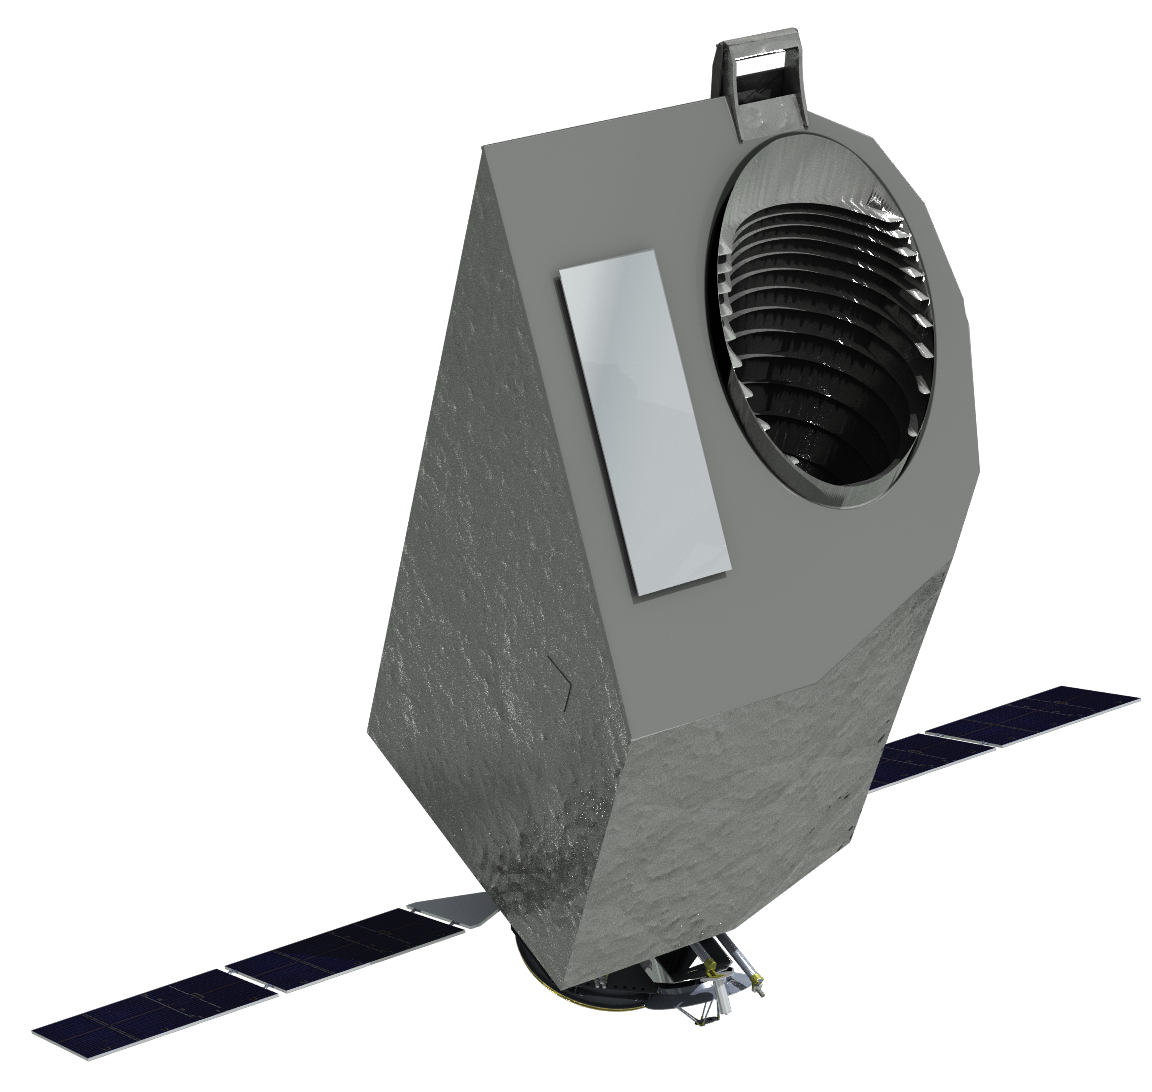
\includegraphics[width=\columnwidth]{figures/UVEXrender}
    \caption{\label{fig:render}A rendering of \ac{UVEX}. Reproduced from the \ac{CSR} and from \citet{2021arXiv211115608K}.}
\end{figure}

\ac{UVEX}'s expected launch in 2030 will be few years after ULTRASAT, but it will be significantly more capable than ULTRASAT: it will take images simultaneously in two bands, it will observe much deeper ($>$25.8~mag over the entire survey), it will have a \ac{PSF} that is well-matched to ground-based follow-up ($\sim1\arcsec$), and it will have an onboard spectrograph. \ac{UVEX} will not just perform a transformative all-sky time-domain \ac{UV} survey. It will also be able to perform \acp{ToO} to follow up \ac{GW} mergers and other multimessenger phenomena (see Fig.~\ref{fig:uvex-tiling}). With its wide \ac{FOV} and two \ac{UV} bandpasses, it should be able to finally discern the physical mechanism of early-time emission in \acp{KN}.

\begin{figure}
    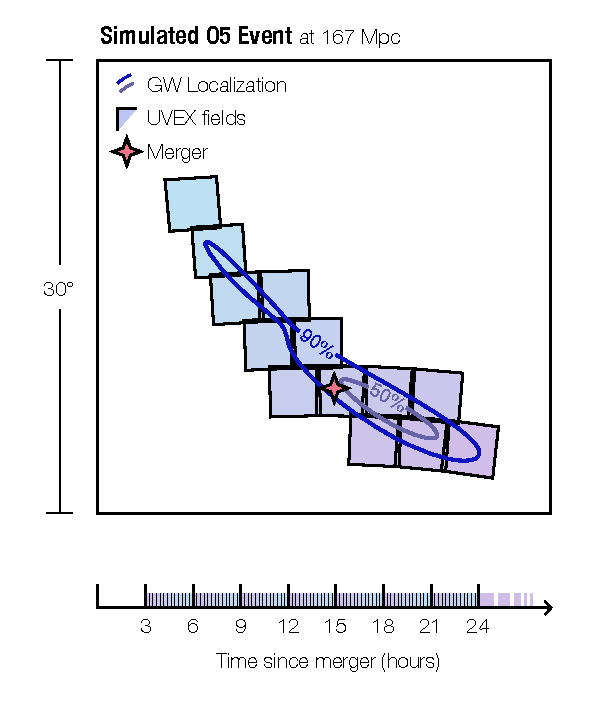
\includegraphics[width=\columnwidth]{figures/uvex-tiling}
    \caption{\label{fig:uvex-tiling}An example of a \ac{ToO} observation sequence with \ac{UVEX} to follow up a \ac{GW} event. Adapted from Fig.~D-8 from the \ac{UVEX} \ac{CSR} submitted to NASA Headquarters, which is also Fig.~14 in \citet{2021arXiv211115608K}.}
\end{figure}

\subsection{A Multi-Mission Multi-Messenger Observation Planning Toolkit}

In \citet{criswell}, we elaborated upon the case for \ac{GW} follow-up with \ac{UVEX} more or less as we presented it to NASA in the \ac{CSR}.
That \ac{UVEX} study leveraged the same \ac{GW} \ac{ToO} analysis and strategy that we had developed for the Dorado study. We envisioned our observation planning software, dorado-scheduling\footnote{\url{https://github.com/nasa/dorado-scheduling}}, as an early draft of what would eventually evolve into real ground software and a part of the guest observer toolkit.
Therefore, the study benefited from an unusual level of fidelity and realism for so early in the mission lifecycle.

The dorado-scheduling package takes into consideration the time-varying \ac{FoR} of the telescope and employs the formalism of \ac{MILP} to find the globally optimal sequence of observations that covers the largest integrated probability within the \ac{GW} localization. Responding to inquiries from the Dorado reviewers about varying extinction and foregrounds, we added to the scheduler the capability to dynamically vary the exposure time of each field to adjust for spatial variations in sensitivity. This code remained on a Git branch, so it was not used in the \ac{UVEX} study.

Additionally, dorado-scheduling had the major limitation that it was released under the obscure and anachronistic \ac{NOSA}, which placed severe obstacles to our own collaborators using or contributing to it. Lawyers at \ac{GSFC} continue to require all \ac{GSFC} scientists to employ \ac{NOSA} even though it has has been rejected by the \citet{FSF}, the \citet{NAP25217}, and even the \citet{SMD}. Fortunately, NASA Headquarters intervened in this case and we were permitted to establish a new truly open-source and permissively licensed software project. However, this required a rewrite which took several years.

In this paper, we introduce \ac{M4OPT}. It is released under a permissive, mainstream license (BSD), but it has many other advances over the earlier work:
%
\begin{itemize}
    \item It is designed from the start to support multiple missions, including \ac{UVEX} and ULTRASAT.
    \item It can adjust exposure times given the anticipated absolute magnitude and the three-dimensional \ac{GW} localization distribution in sky position and distance.
    \item It can dynamically vary the exposure time of each field to pierce through spatial variations in foregrounds (zodiacal light, Galactic diffuse emission) and dust extinction.
    \item It can be given the ancicipated absolute magnitude of the source as either a point estimate or a distribution with Gaussian uncertainty.
    \item The dynamic exposure times are made possible by a NumPy \citep{harris2020array} vectorized \ac{ETC} which makes it possible to do large parameter sweeps of synthetic photometry calculations which are otherwise prohibitively slow with synphot \citep{2018ascl.soft11001S} alone.
    \item It models additional spacecraft dynamics effects, including the roll angle of the telescope which is determined by solar power requirements.
\end{itemize}

\section{Basics of \ac{MILP}}

\Ac{LP} is a mathematical optimization formalism in which one represents an objective as a linear combination of decision variables, subject to constraints that take the form of a system of linear inequalities. The canonical form a \ac{LP} is
%
\begin{alignat*}{4}
    \text{Find}\quad && &\mathbf{x} \in \mathbb{R}^N \\
    \text{that maximizes}\quad && \mathbf{c}^\mathsf{T} &\mathbf{x} \\
    \text{subject to}\quad && \mathbf{A} &\mathbf{x} \leq 0 \\
    \text{and}\quad && &\mathbf{x} \geq 0.
\end{alignat*}
%
\ac{LP} is useful for problems of resource allocation and scheduling. If instead of being reals, certain of the decision variables are required to be integers, then the problem is called \acf{MILP}. \ac{MILP} allows one to model situations where some decision variables represent alternative courses of action or where some constraints are Boolean in nature.

The classic \ac{MWC} has a \ac{MILP} representation that forms the basis of our scheduler. In \ac{MWC}, one has a finite sequence of real-valued weights, $(w_j)_j$ and a finite set of sets, $S = \{S_i\}_i$, over the integers, $\forall i: S_i \subset \mathbb{Z}$. The objective is to find a subset $S^\prime \subseteq S$, with a maximum cardinality $|S^\prime| \leq k$, that maximizes the sum over all of the weights $\sum_{j \in \cup S^\prime} w_j$. This is illustrated in Fig.~\ref{fig:max-weighted-coverage}. The \ac{MWC} has a straightforward \ac{MILP} representation:
%
\begin{align*}
\text{Maximize}\quad &\sum_j y_j w_j \\
\text{subject to the constraints}\quad &\sum_i x_i \leq k \\
\text{and}\quad &\sum_{\mathclap{i \mid j \in S_i}} x_i \geq y_j.
\end{align*}

\begin{figure}
    \centering
    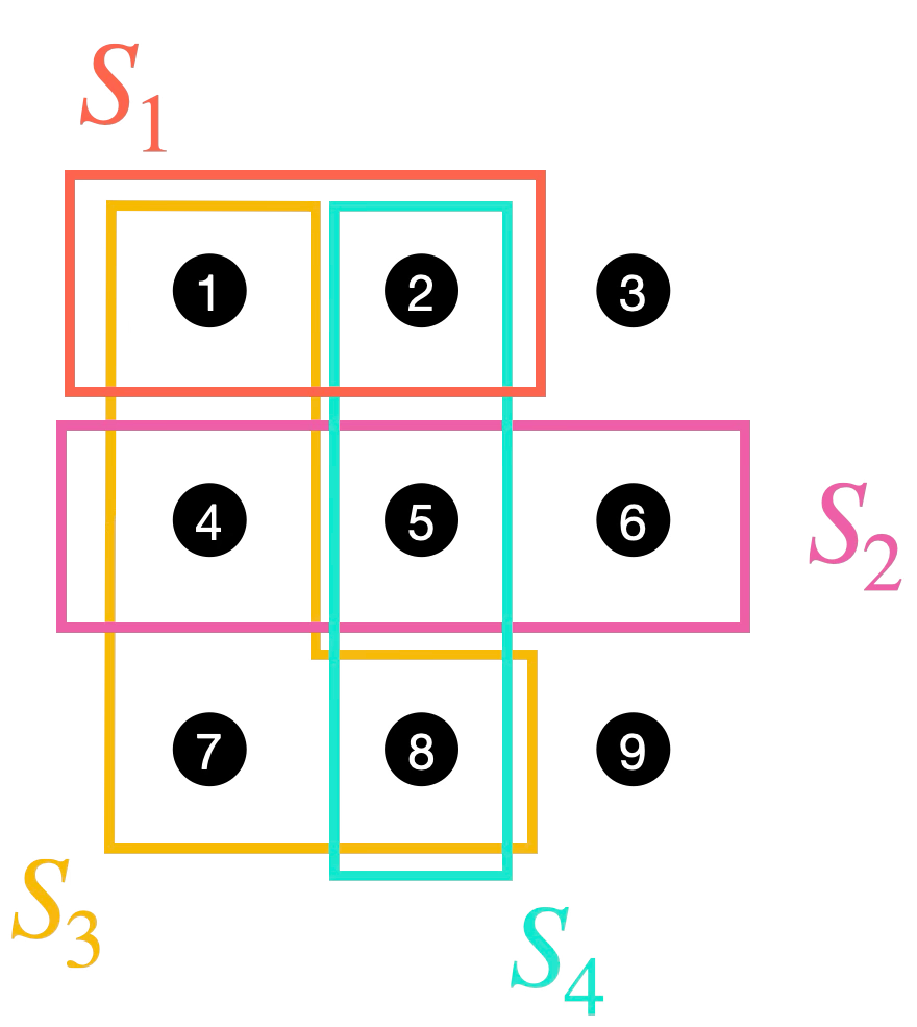
\includegraphics[width=0.6\columnwidth]{figures/max-weighted-coverage}
    \caption{\label{fig:max-weighted-coverage}Illustration of the maximum weighted coverage problem. Four sets $S = \{S_1, S_2, S_3, S_4\}$ are represented as regions with colored borders. The elements of those sets are represented by black numbered circles.}
\end{figure}

Application to HEALPix coverage... Fig.~\ref{fig:overlapping-fields}.

\begin{figure}
    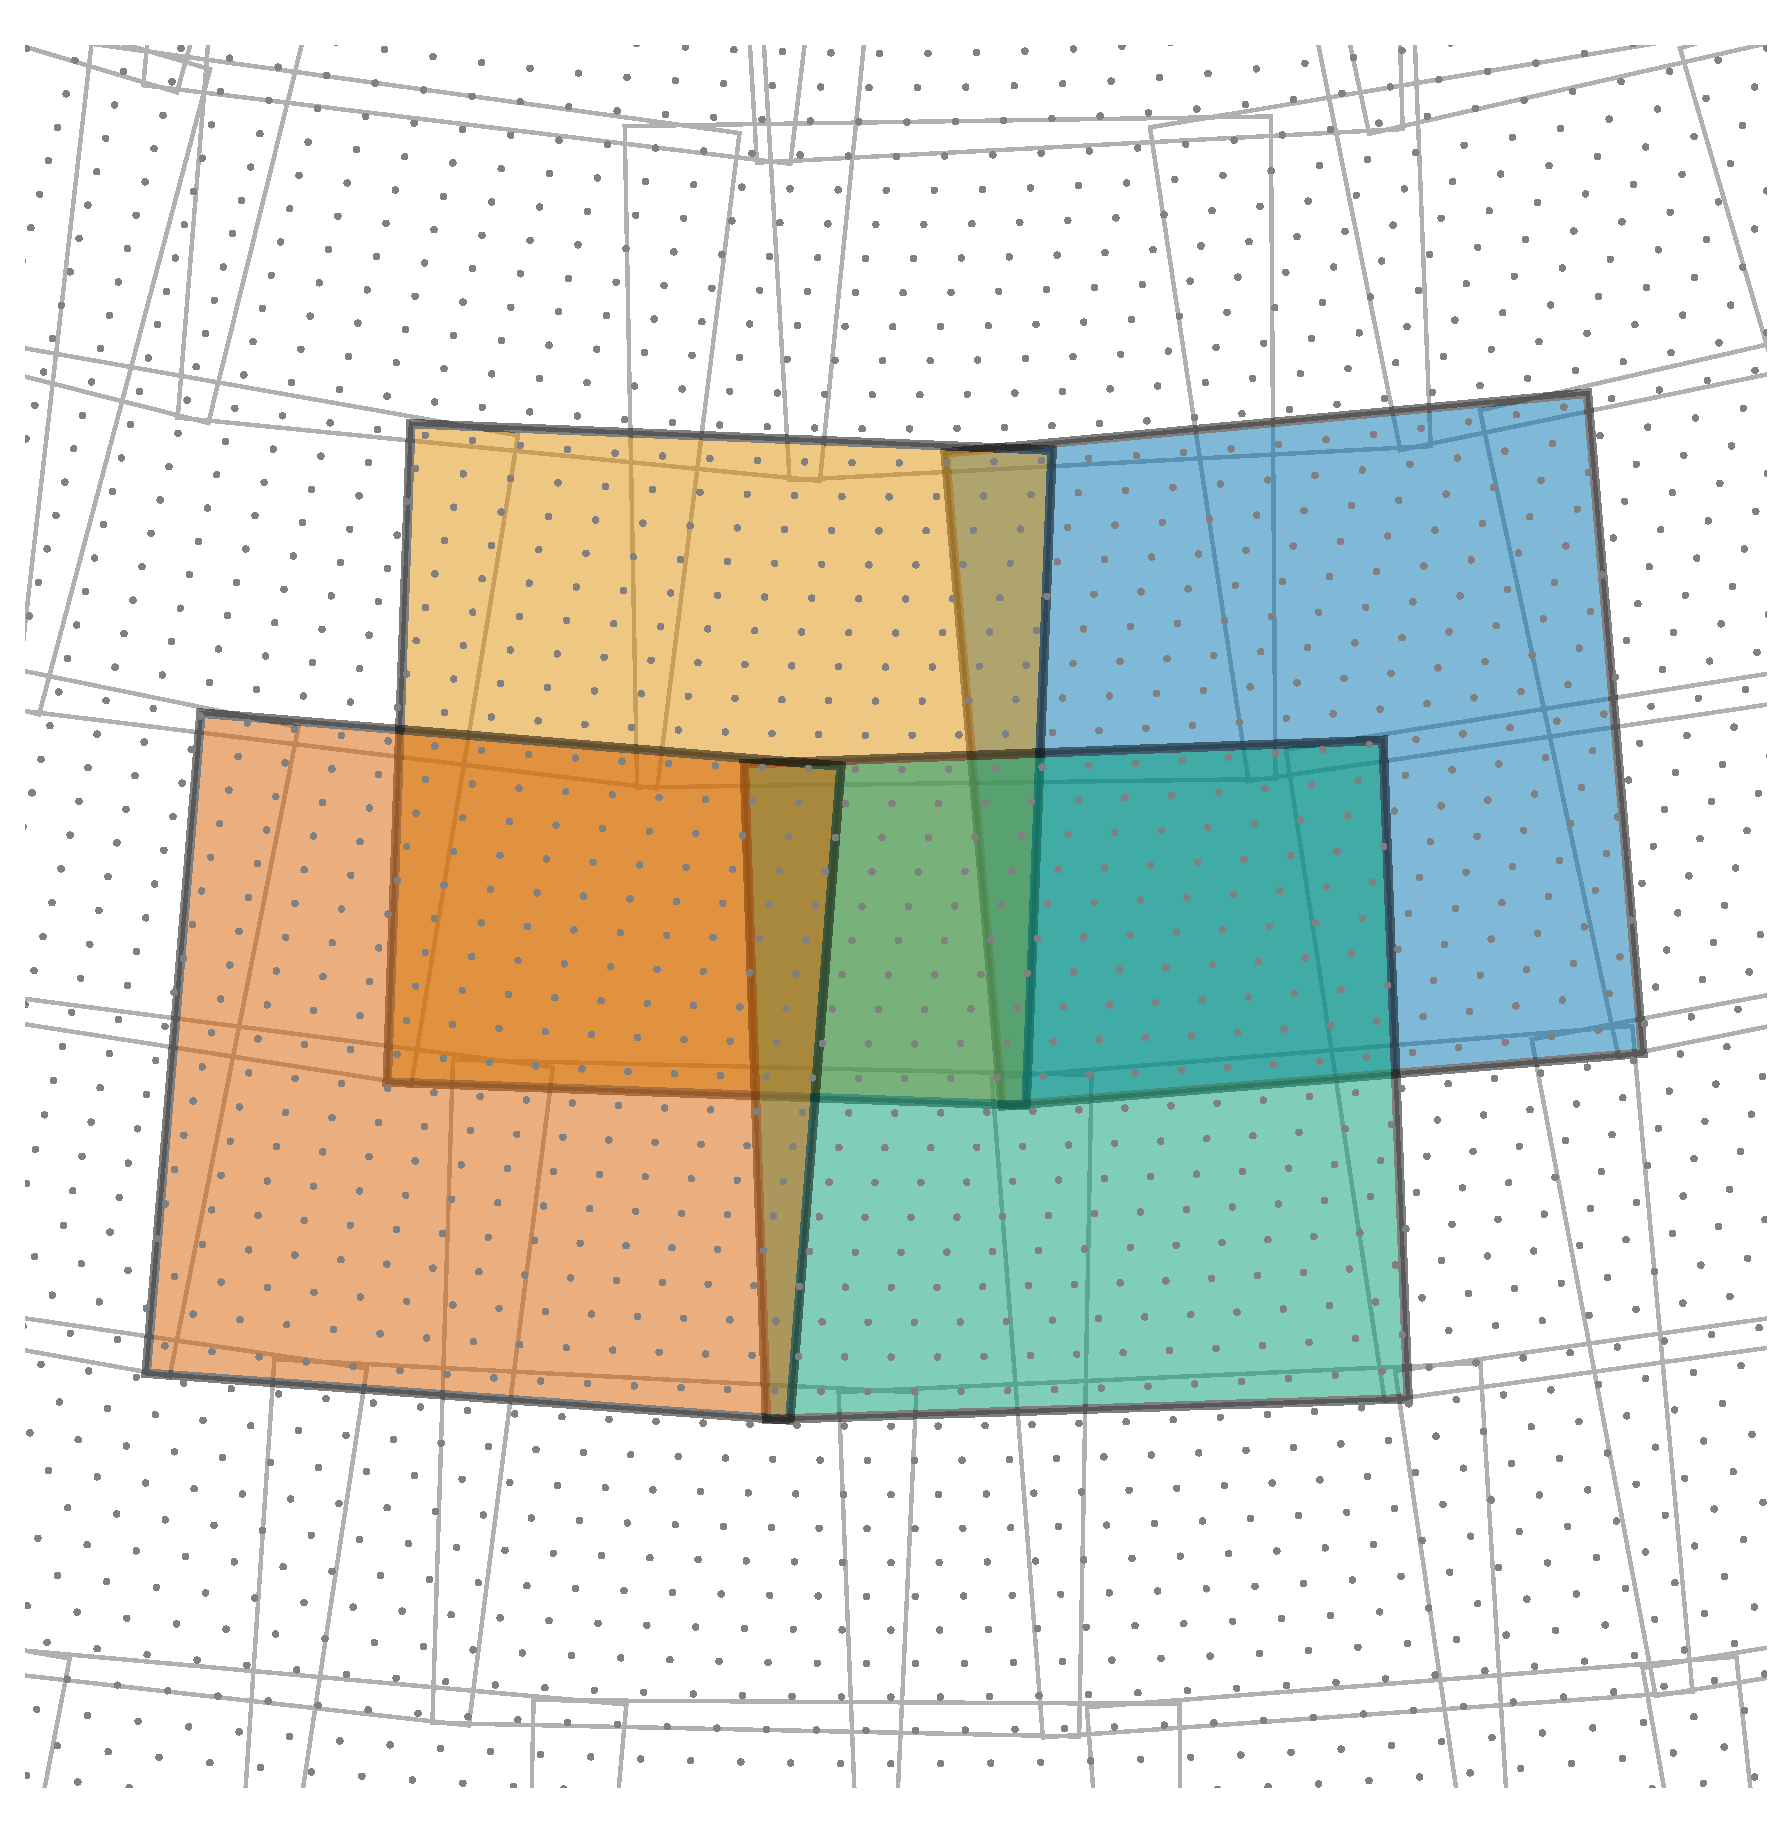
\includegraphics[width=\columnwidth]{figures/overlapping-fields}
    \caption{\label{fig:overlapping-fields}The maximum weighted coverage problem applied to overlapping HEALPix footprints.}
\end{figure}

\section{Multimessenger Follow-Up as an \ac{MILP} Problem}

Here we document our representation of the multimessenger follow-up problem as a mixed integer linear program.

\subsection{Problem 1: Fixed Exposure Time}

We receive a HEALPix probability sky map that describes the probability distribution of the true but unknown position of a target of interest as a function of position on the sky. There is a delay between the time that the event occurred and when we can start observations due to the time it takes to uplink commands to the spacecraft, and there is a deadline by which we must complete our observations.

Our telescope can observe any of a set of $n_J$ fields at predetermined sky locations in order to tile the sky map. For each field that we select, our telescope must visit the field at least $n_K$ times. We have a cadence requirement: each visit of a given field must occur at least a time $\gamma$ after the previous visit.

Every visit takes a certain amount of exposure time, and it takes a known amount of time to slew between different fields. We may only a visit a field when it is within the field of regard, the region that constrains where the telescope may point at any given instant of time.

\subsubsection{Data Preparation}

\begin{enumerate}
    \item Construct a discrete 1D grid of times that stretch from the delayed start of observations up to the deadline.
    \item Propagate the orbit of the spacecraft to calculate the position of the spacecraft at each time step.
    \item For each field and each time step, test whether the field is within the instantaneous field of regard, creating an observability bit map.
    \item Transform the observability bit map into a list of time segments during which each field is observable.
    \item Discard segments shorter than the exposure time.
    \item Discard fields that have no observable segments.
    \item For each field, find the HEALPix pixel indices that are within the field's footprint.
    \item Select the 50 fields that contain the greatest probability.
    \item Discard pixels that are not contained in any field.
    \item Calculate the slew times between fields.
\end{enumerate}

\subsubsection{Problem Setup}

\begin{alignat*}{3}
\intertext{\it Index sets ---}
    &\text{pixels}&
        I =& \{0, 1, \dots, n_I - 1\} \\
    &\text{fields}&
        J =& \{0, 1, \dots, n_J - 1\} \\
    &\text{visits}&
        K =& \{0, 1, \dots, n_K - 1\} \\
    &\text{observable segments}&
        (M_j =& \{0, 1, \dots, {n_M}_j\})_{j \in J} \\
    &\text{fields containing pixel $i$}&
        (J_i =& \{0, 1, \dots, {n_J}_i\})_{i \in I} \\
\intertext{\it Parameters ---}
    &\text{probability of pixel $i$}&
        (\rho_i&)_{i \in I} \\
    &\text{slew time from field $j$ to $j^\prime$}&
        (\sigma_{jj^\prime}&)_{j \in J, j^\prime \in J} \\
    &\text{start times of segments}&
        (\alpha_{jm}&)_{j \in J, m \in M} \\
    &\text{end times of segments}&
        (\omega_{jm}&)_{j \in J, m \in M} \\
    &\text{exposure time}&
        \epsilon& \\
    &\text{cadence, time between visits}&
        \gamma& \\
    &\text{delay}&
        \beta& \\
    &\text{deadline}&
        \delta& \\
\intertext{\it Binary decision variables ---}
    &\text{pixel $i$ is in any selected field}&
        (p_i&)_{i \in I} \\
    &\text{field $j$ is selected}&
        (r_j&)_{j \in J} \\
    &\text{field $j$ visit $k$ is in segment $m$}&
        (s_{jkm}&)_{j \in J, k \in K, m \in M \mid {n_M}_j > 1} \\
\intertext{\it Continuous decision variables ---}
    &\text{mid time of field $j$ visit $k$}& (t_{jk}&)_{j \in J, k \in K}
\end{alignat*}

\subsubsection{Constraints}

\paragraph{Containment}
Only count pixels that are in one or more selected fields.
%
\begin{equation}
    \label{eq:fixed-exptime-constraint-containment}
    \forall i :\quad p_i \leq \sum_{j \in J_i} r_j
\end{equation}

\paragraph{Cadence}
If a field is selected for observation, then enforce a minimum time between visits.
%
\begin{equation}
    \label{eq:fixed-exptime-constraint-cadence}
    \forall k > 1 ,\; j :\quad t_{jk} - t_{j,k-1} \geq (\epsilon + \gamma) r_j
\end{equation}

\paragraph{No overlap}
Observations cannot overlap in time; they must be separated by at least the exposure time plus the slew time.
%
\begin{multline}
    \label{eq:fixed-exptime-constraint-no-overlap}
    \forall j^\prime > j,\; k ,\; k^\prime : \\ \left|t_{jk} - t_{j^\prime k^\prime}\right|  \geq \left(\sigma_{jj^\prime} + \epsilon\right) \left( r_j + r_{j^\prime} - 1\right)
\end{multline}

\paragraph{\ac{FoR}}
An observation of a field can only occur while the coordinates of the field are within the \ac{FoR}. For fields that have one observable segment (${n_M}_j = 1$), this constraint is simpy an inequality:
%
\begin{equation}
    \label{eq:fixed-exptime-constraint-for-one}
    \forall j ,\; k \;, m \mid {n_M}_j = 1 :\quad \alpha_{jm} + \epsilon / 2 \leq t_{jk} \leq \omega_{jm} - \epsilon / 2
\end{equation}
%
For fields that have more than one observable segment (${n_M}_j > 1$), we use the decision variable $s_{jkm}$ to determine which inequality is satisfied:
%
\begin{alignat}{2}
    \label{eq:fixed-exptime-constraint-for-many}
    \forall j ,\; k \;, &m \mid {n_M}_j > 1 : \nonumber \\
    &s_{jkm} = 1 \;\Rightarrow\; \alpha_{jm} + \epsilon / 2 \leq t_{jk} \leq \omega_{jm} - \epsilon / 2 \\
    &\sum_m s_{jkm} \geq 1
\end{alignat}

\subsubsection{Cuts}

\paragraph{Total exposure time}
Although it is implied by other constraints, the constraint that the total exposure time cannot exceed the total available time is found to speed up the search.
%
\begin{equation}
    \label{eq:fixed-exptime-cut-total-time}
    \sum_{j \in J} r_j \leq \frac{\delta - \beta}{\epsilon n_K}
\end{equation}

\subsubsection{Objective}

Maximize the sum of the probability of all of the pixels that are contained within selected fields:
%
\begin{equation}
    \label{eq:fixed-exptime-objective}
    \sum_{i \in I} \rho_i p_i
\end{equation}

\subsection{Problem 2: Variable Exposure Time}

In this variation, we have a sky map of the exposure time required to detect the source as a function of its position on the sky. We permit the exposure time to vary for each field. A given pixel counts toward the objective value only if the exposure time of a field that contains that pixel exceeds the pixel's exposure time.

\subsubsection{Problem Setup}

\begin{alignat*}{3}
\intertext{\it Additional parameters ---}
    &\text{min exposure time to detect a source in pixel $i$}\quad&
        (\epsilon_i)_{i \in I} \\
    &\text{min allowed exposure time}\quad&
        \epsilon_\mathrm{min} \\
    &\text{max allowed exposure time}\quad&
        \epsilon_\mathrm{max}
\intertext{\it Additional, semicontinuous decision variables ---}
    &\text{exposure time of field $j$}\quad& \\
    &\qquad\left(e_j\right)_{j \in J}, \forall j \in J : e_j = 0 \text{ or } \epsilon_\mathrm{min} \leq e_j \leq \epsilon_\mathrm{max}
\end{alignat*}

\subsubsection{Constraints}

The constraints are slightly different.

\paragraph{Depth}
Only count pixels that are observed to sufficient exposure time.
%
\begin{equation}
    \label{eq:variable-exptime-constraint-depth}
    \forall i \in I :\quad p_\mathrm{i} = 1 \Rightarrow \max_{j \in J_i} e_{j} \geq \epsilon_i
\end{equation}

\paragraph{Exposure time}
If a field's exposure time is nonzero, then it is selected for observation.
%
\begin{equation}
    \label{eq:variable-exptime-constraint-exptime}
    \forall j \in J :\quad \epsilon_\mathrm{max} r_j \geq e_\mathrm{j}
\end{equation}

\paragraph{Cadence}
This is similar to Eq.~(\ref{eq:fixed-exptime-constraint-cadence}), except that we replace the right-hand side of the inequality.
%
\begin{equation}
    \label{eq:variable-exptime-constraint-cadence}
    \forall k > 1 ,\; j :\quad t_{jk} - t_{j,k-1} \geq \gamma r_j + e_j
\end{equation}

\paragraph{No overlap}
This is also similar to Eq.~(\ref{eq:fixed-exptime-constraint-no-overlap}), except with a slightly different right-hand side.
%
\begin{multline}
    \label{eq:variable-exptime-constraint-no-overlap}
    \forall j^\prime > j ,\; k ,\; k^\prime : \\ \left|t_{jk} - t_{j^\prime k^\prime}\right|  \geq \sigma_{jj^\prime} \left( r_j + r_{j^\prime} - 1\right) + (e_j + e_\mathrm{j^\prime}) / 2
\end{multline}

\paragraph{\ac{FoR}}
This is similar to Eqs.~(\ref{eq:fixed-exptime-constraint-for-one},~\ref{eq:fixed-exptime-constraint-for-many}), except that we replace $\epsilon$ with $e_j$. For fields that have one observable segment:
%
\begin{multline}
    \label{eq:variable-exptime-constraint-for-one}
    \forall j ,\; k \;, m \mid {n_M}_j = 1 : \\ \alpha_{jm} + e_j / 2 \leq t_{jk} \leq \omega_{jm} - e_j / 2
\end{multline}
%
For fields that have more than one observable segment:
%
\begin{alignat}{2}
    \label{eq:variable-exptime-constraint-for-many}
    \forall j ,\; &k \;, m \mid {n_M}_j > 1 : \nonumber \\
    &s_{jkm} = 1 \;\Rightarrow\; \alpha_{jm} + e_j / 2 \leq t_{jk} \leq \omega_{jm} - e_j / 2 \\
    &\sum_m s_{jkm} \geq 1
\end{alignat}

\subsubsection{Cuts}

\paragraph{Total exposure time}
Replace Eq.~(\ref{eq:fixed-exptime-cut-total-time}) with:
%
\begin{eqnarray}
    \label{eq:ariable-exptime-cut-total-time}
    \sum_{j \in J} r_j &\leq& \frac{\delta - \beta}{\epsilon_\mathrm{min} n_K} \\
    \sum_{j \in J} e_j &\leq& \frac{\delta - \beta}{n_K}
\end{eqnarray}

\subsubsection{Objective}

Same as above.

\subsection{Problem 3: Variable Exposure Time with Prior Distribution of Absolute Magnitude}

In this variation, we don't know the precise absolute magnitude $X$ of the source. In the case of kilonovae, our prior knowledge about the absolute magnitude is scant; for the sake of mathematical convenience, we assume that the absolute magnitude has a normal distribution, $X \sim~ \mathcal{N}[\mu_X, \sigma_X]$. We need to compute the distribution of \textit{apparent} magnitudes $x$ in order to determine the probability of detection as a function of exposure time for each pixel.

Gravitational-wave sky maps provide the posterior distribution of distance, as a parametric ansatz distribution \citep{2016ApJ...829L..15S,2016ApJS..226...10S},
%
$$
    p(r) = \frac{N}{\sqrt{2 \pi}\sigma} \exp\left[-\frac{1}{2}\left(\frac{r - \mu}{\sigma}\right)^2\right] r^2,
$$
%
with the location parameter $\mu$, scale parameter $\sigma$, and normalization $N$ tabulated for each pixel. This is an inconvenient distribution for integration, so instead we construct a log-normal distance distribution with the same mean and standard deviation as the ansatz distribution.

We calculate the mean $m$ and standard deviation $s$ from $\mu$ and $\sigma$ using the function \verb|parameters_to_moments| from ligo.skymap\footnote{\url{https://lscsoft.docs.ligo.org/ligo.skymap/distance/}}. Then, the location and scale parameters of the log-normal distribution are given by
%
\begin{eqnarray}
    \label{eq:log-distance-parameters}
    \mu_{\ln r} &=& \ln m - \frac{1}{2} \ln \left(1 + \frac{s^2}{m^2}\right) \\
    {\sigma_{\ln r}}^2 &=& \ln \left(1 + \frac{s^2}{m^2}\right).
\end{eqnarray}

The logarithm of the distance then has the distribution $\ln r \sim \mathcal{N}[\mu_{\ln r}, \sigma_{\ln r}]$. The apparent magnitude is related to the absolute magnitude through $x = X + 5 \log_{10} r + 25$, assuming that $r$ is in the units of Mpc. Therefore the apparent magnitude has the distribution $x \sim \mathcal{N}[\mu_x, \sigma_x]$, with
%
\begin{eqnarray}
    \label{eq:appmag-parameters}
    \mu_x &=& \mu_X + \left(\frac{5}{\ln 10}\right) \mu_{\ln r} + 25 \\
    {\sigma_x}^2 &=& {\sigma_{X}}^2 + \left(\frac{5}{\ln 10}\right)^2 {\sigma_{\ln r}}^2.
\end{eqnarray}

With this Gaussian distribution of apparent magnitudes, we can now calculate the detection efficiency for each pixel: the probability that we detect the source assuming that the source is in that pixel, as a function of exposure time. For the purpose of implementation of this function in a MILP, we approximate it with a piecewise linear function, as illustrated in Fig~\ref{fig:piecewise-linear-exptime}.

\begin{figure}
    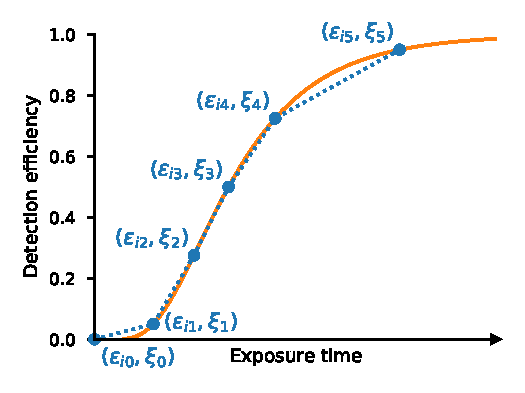
\includegraphics[width=\columnwidth]{figures/piecewise-linear-exptime}
    \caption{\label{fig:piecewise-linear-exptime}Piecewise linear approximation of the detection efficiency for a given pixel. In this example, we have assumed that the exposure time is inversely proportional to the square root of the flux, valid for sky background dominated imaging.}
\end{figure}

\subsubsection{Additional Data Preparation}

\begin{enumerate}
    \item Use the function \verb|parameters_to_moments| and Eqs.~(\ref{eq:log-distance-parameters},~\ref{eq:appmag-parameters}) to calculate the mean and standard deviation of the apparent magnitude in each pixel.
    \item Select desired quantiles for the approximation of the detection efficiency curve: for example, $(0, 0.05 , 0.275, 0.5  , 0.725, 0.95)$. For each pixel, calculate the exposure time required to achieve the specified detection efficiencies.
\end{enumerate}

\subsubsection{Problem Setup}

\begin{alignat*}{3}
\intertext{\it Additional index sets ---}
    &\text{indices of quantiles}&\quad
        N = \{0, 1, \dots, n_N\} \\
\intertext{\it Additional parameters ---}
    &\text{quantiles of detection efficiency}&\quad
        (\xi_n)_{n \in N} \\
    &\text{exposure time of quantiles}&\quad
        (\epsilon_{in})_{i \in I, n \in N} \\
    &\text{piecewise linear functions}&\quad
        (f_i: \mathbb{R}_{\geq 0} \rightarrow [0, 1])_{i \in I}
\end{alignat*}


\subsubsection{Additional Constraints}

\paragraph{Depth}
Replace Eq.~\ref{eq:variable-exptime-constraint-depth} with:
%
$$
    \forall i \in I :\quad \max_{j \in J_i} e_{j} \geq f_i(p_\mathrm{i})
$$

\subsubsection{Objective}

Same as above.

\section{Case study: GW observations with UVEX}

Here is the setup of our case study.

\paragraph{\Ac{GW} localizations}
We started with the same simulated \ac{GW} localizations as \citet{criswell}, which covers LIGO, Virgo, and KAGRA's fifth~(O5) and sixth~(O6) observing runs. The data are publicly archived in \cite{r_weizmann_2024_14142970}. These simulated events were generated using the same methodology as \citet{2022ApJ...924...54P} and \citet{2023ApJ...958..158K}, except that the \ac{S/N} threshold for \ac{GW} detection is set to~10. The localizations were generated with the rapid localization engine BAYESTAR \citep{2016PhRvD..93b4013S} and consist of 3D posterior probability distributions of sky location and luminosity distance \citep{2016ApJ...829L..15S,2016ApJS..226...10S}.

\paragraph{\Ac{KN} absolute magnitude}
Appendix~E.2 of \citet{2021arXiv211115608K} specifies fiducial parameter ranges for radioactively-powered or shock-powered \ac{KN} models and 90\% credible intervals for the absolute magnitude in each band. These absolute magnitude ranges are reproduced in the Table~\ref{tab:kn-abs-mag}. \ac{UVEX} obseves in both the \ac{NUV} and \ac{FUV} filters simultaneously. In orer to achieve a detection in at least one filter, regardless of the model, we should plan obsevations using the fainter of the two models and the brighter of the two bands: the nucleosynthesis-powered model in NUV, with an absolute magnitude range of $[-15.6, -12.4]$. Assuming that this is the 90\% credible interval of a Gaussian distribution, the absolute magnitude has the approximate distribution
%
\begin{equation}
    M_\mathrm{NUV} \sim \mathcal{N}(-14, 1).
\end{equation}

\begin{deluxetable}{lcc}
    \tablecaption{\label{tab:kn-abs-mag}Ranges of peak absolute magnitudes of \acp{KN}. Adapted from \citet{2021arXiv211115608K} Appendix E.2.}
    \tablehead{
        & \multicolumn2c{absolute magnitude range} \\
        \colhead{Model} & \colhead{NUV} & \colhead{FUV}
    }
    \startdata
    Nucleosynthesis powered & [-15.6, -12.4] & [-17.8, -15.3] \\
    Shock powered & [-14.5, -10.2] & [-17.9, -15.0]
    \enddata
\end{deluxetable}

\paragraph{Follow-up time window}
\citet{criswell} required a single epoch of \ac{UVEX} observations to take 3~hours or less. To match this choice, we configure \ac{M4OPT} to plan two visits of each field with a minimum cadence of 30~min between repeated visits, with a total elapsed time limit of 6~hours. 

\paragraph{Exposure time}
The exposure time is allowed to vary adaptively for each field, with a minimum exposure time of $\epsilon_\mathrm{min} = 300$~s. The minimum exposure time corresponds to a single standard \ac{UVEX} imaging exposure. (A standard survey dwell consists of 3 consecutive stacked 300~s exposures.)

\paragraph{FOV}
Like most space telescopes, \ac{UVEX} has solar panels that rotate on a \ac{SADA} perpendicular to the telescope boresight (see Fig.~\ref{fig:render}). The position angle of observations is fixed to the nominal roll angle that allows the spacecraft to orient the solar panels perpendicular to the Sun while keeping the cold side of the spacecraft facing away from the Sun. For any given position, the roll angle goes through one revolution per year. For targets at the ecliptic poles, the nominal roll angle varies linearly with time. For targets in the ecliptic plane, the nominal roll angle flips by 180° at the solstices. At all intermediate ecliptic latitudes, the roll angle oscillates smoothly in a manner that interpolates between these extremes (see Fig.~\ref{fig:nominal-roll}). Because the roll angle changes slowly on the timescale of a day, we calculate the nominal roll angle for each field at the time of the event, and leave it fixed at that value for the duration of the observing plan.

\begin{figure}
    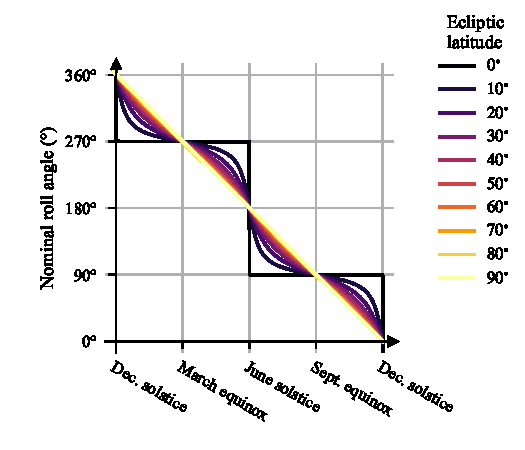
\includegraphics[width=\columnwidth]{figures/nominal-roll}
    \caption{\label{fig:nominal-roll}Nominal roll angle as a function of time for selected ecliptic latitudes.}
\end{figure}

We discretize the footprint of the \ac{UVEX} \ac{FOV} on a HEALPix grid with $n_\mathrm{side} = 128$ (see Fig.~ref\{fig:fov).

\begin{figure}
    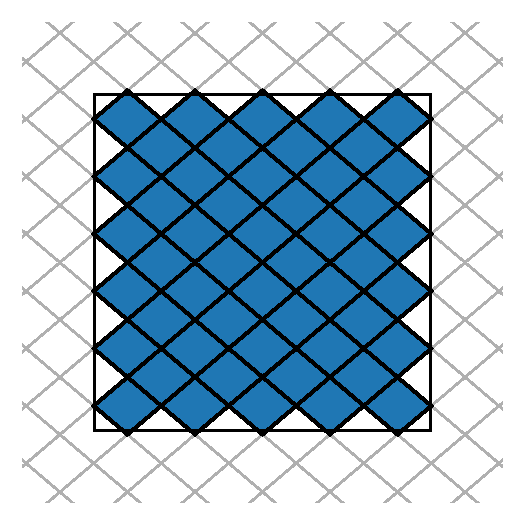
\includegraphics[width=\columnwidth]{figures/fov}
    \caption{\label{fig:fov}The footprint of the \ac{UVEX} \ac{FOV} discretized on a HEALPix grid with $n_\mathrm{side} = 128$.}
\end{figure}

\paragraph{Run duration}
As in \citet{criswell}, we assumed 1.5~years of overlap between the \ac{UVEX} prime mission and the \ac{GW} observing run.

\paragraph{Follow-up selection criterion}
We ran \ac{M4OPT} on all simulated events. We considered events selected for follow-up with \ac{UVEX} if the scheduler's objective values $P$ was less than $P^* = 0.1$. Although the decision of whether to execute a \ac{ToO} is based solely on the scheduler's objective value, we can predict an analytical threshold for triggering on an event based on the area of its $Q$th credible region and its luminosity distance $d_\mathrm{L}$:
%
\begin{eqnarray}
    d_\mathrm{L} &<& d_\mathrm{L}^* = 10^{\frac{1}{5}(x^* - \mu_X + \sigma_X \Phi^{-1}(1-P^*) - 25)}\,\mathrm{Mpc} \label{eq:threshold-distance} \\
    A_Q &<& A_Q^* = \left(\frac{\Psi^{-1}(Q)}{\Psi^{-1}(P^*)}\right)^2 \left(\frac{\delta - \beta}{\epsilon_\mathrm{min} n_K}\right)A_\mathrm{FOV} \label{eq:threshold-area} \\
    \frac{A_Q}{A_\mathrm{FOV}} &<& \left(\frac{d_\mathrm{L}}{d_\mathrm{L}^*}\right)^{-4} \label{eq:threshold-area-distance}
\end{eqnarray}
%
where $x^*$ is the faintest limiting magnitude at any point on the sky, $A_\mathrm{FOV}$ is the area of the \ac{FOV}, $\Phi(x)$ is the inverse of the \ac{CDF} of the standard normal distribution, and $\Psi^{-1}(x) = -2\ln(1 - x)$ is the inverse of the \ac{CDF} of a $\chi^2$ distribution with 2 degrees of freedom.

The results are shown in Fig~\ref{fig:area-distance}. The expected numbers of events selected for follow-up and detected are shown in Table~\ref{tab:selected-detected}.

\begin{figure*}
    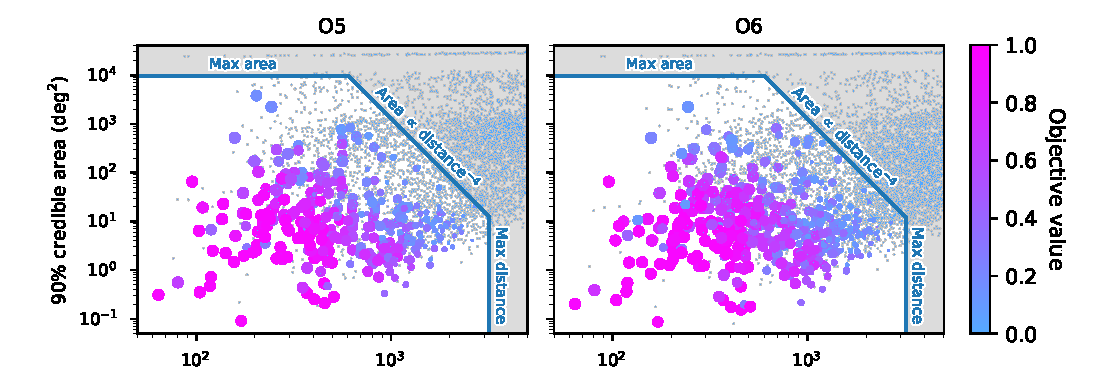
\includegraphics[width=\textwidth]{figures/area-distance}
    \caption{\label{fig:area-distance}90\% credible area and distance of simulated \ac{GW} events. Events that were selected for follow-up with \ac{UVEX} are represented by colored dots, with the color of the dot representing the scheduler objective value and the area of the dot the detection probability. Events that were not selected for follow-up are marked with gray dots. The blue boundary represents the analytical predictor of the detection threshold given by Eqs.~(\ref{eq:threshold-distance},~\ref{eq:threshold-area},~\ref{eq:threshold-area-distance}).}
\end{figure*}

\begin{deluxetable}{lcc}
    \tablecaption{\label{tab:selected-detected}Expected number of events.}
    \tablehead{& O5 & O6}
    \startdata
    Number of events selected & $51_{-31}^{+67}$ & $72_{-42}^{+93}$ \\
Number of events detected & $26_{-16}^{+35}$ & $38_{-23}^{+51}$

    \enddata
\end{deluxetable}

\section{Conclusion}

\begin{acknowledgments}
This work was performed in part at the Aspen Center for Physics, which is supported by \ac{NSF} grant PHY-2210452.

This work used Expanse at \ac{SDSC} through allocation AST200029, ``Towards a complete catalog of variable sources to support efficient searches for compact binary mergers and their products,'' from the \ac{ACCESS} program, which is supported by \ac{NSF} grants \#2138259, \#2138286, \#2138307, \#2137603, and \#2138296.
\end{acknowledgments}

\vspace{5mm}
\software{
    astropy \citep{2013A&A...558A..33A,2018AJ....156..123A},
    astroquery \citep{2019AJ....157...98G},
    dust\_extinction \citep{2024JOSS....9.7023G},
    dustmaps \citep{2018JOSS....3..695M},
    HEALPix \citep{2005ApJ...622..759G},
    healpy \citep{2019JOSS....4.1298Z},
    ligo.skymap \citep{2016PhRvD..93b4013S,2016ApJ...829L..15S,2016ApJS..226...10S},
    NumPy \citep{harris2020array},
    sympy \citep{10.7717/peerj-cs.103},
    synphot \citep{2018ascl.soft11001S}}

\bibliography{m4opt}{}
\bibliographystyle{aasjournal}

\end{document}
